\section{Regla de la Cadena}

En una variable, si $z = f(x)$ y $x = g(t)$, entonces $\dfrac{dz}{dt} = \dfrac{dz}{dx}\dfrac{dx}{dt}$. En varias variables, la misma idea se generaliza: cuando $z$ depende de varias variables intermedias, la derivada total respecto al parámetro final es la suma de las contribuciones de cada camino en el árbol de dependencias.

\subsection{Diagrama de árbol}

El diagrama de árbol es una representación de las relaciones de dependencia entre las variables de una composición. Cada nodo representa una variable, y cada arista lleva la derivada (parcial u ordinaria) de la variable superior respecto a la inferior. La regla de la cadena opera sobre este diagrama de la siguiente manera: para obtener la derivada de la variable raíz respecto a una variable hoja, se identifican todos los caminos que las unen, se multiplican las derivadas a lo largo de cada camino y se suman los resultados.

El diagrama correspondiente a $z = f(x, y)$ con $x = x(t)$, $y = y(t)$ es:

\begin{center}
\shorthandoff{>}
\begin{tikzpicture}[every node/.style={font=\small}]
    \node (z)  at ( 0,  0) {$z$};
    \node (x)  at (-2, -2) {$x$};
    \node (y)  at ( 2, -2) {$y$};
    \node (t1) at (-2, -4) {$t$};
    \node (t2) at ( 2, -4) {$t$};

    \draw[->, thick] (z)  -- (x)
        node[midway, above left,  font=\scriptsize, fill=white, inner sep=1pt]
        {$\dfrac{\partial z}{\partial x}$};
    \draw[->, thick] (z)  -- (y)
        node[midway, above right, font=\scriptsize, fill=white, inner sep=1pt]
        {$\dfrac{\partial z}{\partial y}$};
    \draw[->, thick] (x)  -- (t1)
        node[midway, left,        font=\scriptsize, fill=white, inner sep=1pt]
        {$\dfrac{dx}{dt}$};
    \draw[->, thick] (y)  -- (t2)
        node[midway, right,       font=\scriptsize, fill=white, inner sep=1pt]
        {$\dfrac{dy}{dt}$};
\end{tikzpicture}
\end{center}

Hay dos caminos de $z$ a $t$: uno a través de $x$ y otro a través de $y$. La regla de la cadena suma ambas contribuciones:
\[
\frac{dz}{dt} = \frac{\partial z}{\partial x}\frac{dx}{dt} + \frac{\partial z}{\partial y}\frac{dy}{dt}
\]

Cuando las variables intermedias dependen a su vez de varias variables, el diagrama se expande. Para $z = f(x, y)$ con $x = x(s, t)$, $y = y(s, t)$:

\begin{center}
\shorthandoff{>}
\begin{tikzpicture}[every node/.style={font=\small}]
    \node (z)  at ( 0,  0)  {$z$};
    \node (x)  at (-3, -2)  {$x$};
    \node (y)  at ( 3, -2)  {$y$};
    \node (sx) at (-4, -4)  {$s$};
    \node (tx) at (-2, -4)  {$t$};
    \node (sy) at ( 2, -4)  {$s$};
    \node (ty) at ( 4, -4)  {$t$};

    \draw[->, thick] (z)  -- (x)
        node[midway, above left,  font=\scriptsize, fill=white, inner sep=1pt]
        {$\dfrac{\partial z}{\partial x}$};
    \draw[->, thick] (z)  -- (y)
        node[midway, above right, font=\scriptsize, fill=white, inner sep=1pt]
        {$\dfrac{\partial z}{\partial y}$};
    \draw[->, thick] (x)  -- (sx)
        node[midway, left,        font=\scriptsize, fill=white, inner sep=1pt]
        {$\dfrac{\partial x}{\partial s}$};
    \draw[->, thick] (x)  -- (tx)
        node[midway, right,       font=\scriptsize, fill=white, inner sep=1pt]
        {$\dfrac{\partial x}{\partial t}$};
    \draw[->, thick] (y)  -- (sy)
        node[midway, left,        font=\scriptsize, fill=white, inner sep=1pt]
        {$\dfrac{\partial y}{\partial s}$};
    \draw[->, thick] (y)  -- (ty)
        node[midway, right,       font=\scriptsize, fill=white, inner sep=1pt]
        {$\dfrac{\partial y}{\partial t}$};
\end{tikzpicture}
\end{center}

Para $\partial z/\partial s$ se recorren los caminos $z \to x \to s$ y $z \to y \to s$; para $\partial z/\partial t$ los caminos $z \to x \to t$ y $z \to y \to t$.

\subsection{La regla de la cadena}

\subsubsection{Caso 1: una variable paramétrica}

\begin{mytheorem}{Regla de la cadena: caso 1}
Sea $z = f(x, y)$ diferenciable y sean $x = x(t)$, $y = y(t)$ diferenciables en $t$. Entonces $z$ es diferenciable como función de $t$ y:
\[
\frac{dz}{dt} = \frac{\partial z}{\partial x}\frac{dx}{dt} + \frac{\partial z}{\partial y}\frac{dy}{dt}
\]
\end{mytheorem}

\textbf{Ejemplo.} Sea $z = x^2 + y^2$ con $x = \cos t$, $y = \sin t$. Por la regla de la cadena:
\[
\frac{dz}{dt} = 2x(-\sin t) + 2y(\cos t) = -2\cos t\sin t + 2\sin t\cos t = 0
\]
El resultado es coherente: $z = \cos^2 t + \sin^2 t = 1$ es constante, por lo que su derivada es cero.

\subsubsection{Caso 2: dos variables paramétricas}

\begin{mytheorem}{Regla de la cadena: caso 2}
Sea $z = f(x, y)$ diferenciable y sean $x = x(s, t)$, $y = y(s, t)$ con derivadas parciales continuas. Entonces:
\[
\frac{\partial z}{\partial s} = \frac{\partial z}{\partial x}\frac{\partial x}{\partial s} + \frac{\partial z}{\partial y}\frac{\partial y}{\partial s}
\qquad
\frac{\partial z}{\partial t} = \frac{\partial z}{\partial x}\frac{\partial x}{\partial t} + \frac{\partial z}{\partial y}\frac{\partial y}{\partial t}
\]
\end{mytheorem}

\textbf{Ejemplo.} Sea $z = e^x \sin y$ con $x = st^2$, $y = s^2 t$. Entonces:
\[
\frac{\partial z}{\partial s}
= e^x \sin y \cdot t^2 + e^x \cos y \cdot 2st
= e^{st^2}(t^2 \sin(s^2 t) + 2st\cos(s^2 t))
\]
\[
\frac{\partial z}{\partial t}
= e^x \sin y \cdot 2st + e^x \cos y \cdot s^2
= e^{st^2}(2st\sin(s^2 t) + s^2\cos(s^2 t))
\]

\subsubsection{Caso general}

\begin{mytheorem}{Regla de la cadena general}
Sea $w = f(x_1, \dots, x_m)$ diferenciable y sean $x_i = x_i(t_1, \dots, t_n)$ funciones con derivadas parciales continuas. Para cada $k = 1, \dots, n$:
\[
\frac{\partial w}{\partial t_k}
= \sum_{i=1}^{m} \frac{\partial w}{\partial x_i}\frac{\partial x_i}{\partial t_k}
= \frac{\partial w}{\partial x_1}\frac{\partial x_1}{\partial t_k}
+ \frac{\partial w}{\partial x_2}\frac{\partial x_2}{\partial t_k}
+ \cdots
+ \frac{\partial w}{\partial x_m}\frac{\partial x_m}{\partial t_k}
\]
\end{mytheorem}

La suma recorre todas las variables intermedias $x_i$, y cada término corresponde a uno de los caminos del árbol de dependencias que conecta $w$ con $t_k$.

\textbf{Ejemplo.} Sea $w = xy + yz + xz$ con $x = t\cos t$, $y = t\sin t$, $z = t$. Las derivadas ordinarias de las variables intermedias son $\dot{x} = \cos t - t\sin t$, $\dot{y} = \sin t + t\cos t$, $\dot{z} = 1$. Por la regla de la cadena:
\[
\frac{dw}{dt}
= (y + z)\dot{x} + (x + z)\dot{y} + (y + x)\dot{z}
\]
que se evalúa sustituyendo las expresiones en función de $t$.

\subsection{Derivación implícita}

Cuando una ecuación $F(x, y) = 0$ define $y$ como función diferenciable de $x$, la regla de la cadena permite calcular $dy/dx$ sin necesidad de despejar $y$ explícitamente.

\subsubsection*{Caso $F(x, y) = 0$}

Suponga que la ecuación $F(x, y) = 0$ define implícitamente $y = y(x)$. Al sustituir esa dependencia, el lado izquierdo se convierte en una función de una sola variable:
\[
F\bigl(x,\, y(x)\bigr) = 0 \qquad \text{para todo } x \text{ en un intervalo.}
\]
Como esta identidad se cumple para todo $x$, se puede derivar ambos lados respecto de $x$. El miembro derecho es la constante $0$, cuya derivada es nula. El miembro izquierdo es una composición: $F$ depende de $x$ de dos maneras, directamente a través de su primer argumento e indirectamente a través de $y(x)$. La regla de la cadena para $w = F(x, y)$ con $x = x$ e $y = y(x)$ da:
\[
\frac{d}{dx}F\bigl(x, y(x)\bigr)
= \frac{\partial F}{\partial x}\cdot\frac{dx}{dx} + \frac{\partial F}{\partial y}\cdot\frac{dy}{dx}
= F_x + F_y\,\frac{dy}{dx}.
\]
Igualando a cero, puesto que la identidad deriva a $0$:
\[
F_x + F_y\,\frac{dy}{dx} = 0.
\]
Despejando el término con $dy/dx$ y dividiendo entre $F_y$, válido siempre que $F_y \neq 0$:
\[
F_y\,\frac{dy}{dx} = -F_x
\qquad\Longrightarrow\qquad
\frac{dy}{dx} = -\frac{F_x}{F_y}.
\]

\subsubsection*{Caso $F(x, y, z) = 0$}

Ahora suponga que la ecuación $F(x, y, z) = 0$ define implícitamente $z = z(x, y)$. Sustituyendo, se obtiene la identidad:
\[
F\bigl(x,\, y,\, z(x, y)\bigr) = 0 \qquad \text{para todo } (x, y) \text{ en una región.}
\]
Para hallar $\partial z / \partial x$ se deriva la identidad respecto de $x$ manteniendo $y$ constante. En esta derivada parcial, $x$ interviene directamente en el primer argumento y también a través de $z(x, y)$, mientras que $y$ se trata como constante, de modo que $\partial y / \partial x = 0$. La regla de la cadena da:
\[
\frac{\partial}{\partial x}F\bigl(x, y, z(x,y)\bigr)
= F_x\,\frac{\partial x}{\partial x} + F_y\,\frac{\partial y}{\partial x} + F_z\,\frac{\partial z}{\partial x}
= F_x + F_z\,\frac{\partial z}{\partial x} = 0.
\]
Despejando, con $F_z \neq 0$:
\[
\frac{\partial z}{\partial x} = -\frac{F_x}{F_z}.
\]
De forma simétrica, derivando la identidad respecto de $y$ con $x$ constante, ahora $\partial x / \partial y = 0$:
\[
F_x\,\frac{\partial x}{\partial y} + F_y\,\frac{\partial y}{\partial y} + F_z\,\frac{\partial z}{\partial y}
= F_y + F_z\,\frac{\partial z}{\partial y} = 0
\qquad\Longrightarrow\qquad
\frac{\partial z}{\partial y} = -\frac{F_y}{F_z}.
\]
En ambos casos el patrón es el mismo: la derivada de la variable dependiente respecto de una independiente es el cociente, con signo negativo, entre la parcial de $F$ respecto de esa variable independiente y la parcial de $F$ respecto de la variable dependiente.

\begin{mytheorem}{Derivación implícita}
Si $F(x, y) = 0$ define $y = y(x)$ diferenciable y $F_y \neq 0$, entonces:
\[
\frac{dy}{dx} = -\frac{F_x}{F_y}
\]
Si $F(x, y, z) = 0$ define $z = z(x,y)$ diferenciable y $F_z \neq 0$, entonces:
\[
\frac{\partial z}{\partial x} = -\frac{F_x}{F_z}
\qquad
\frac{\partial z}{\partial y} = -\frac{F_y}{F_z}
\]
\end{mytheorem}

\textbf{Ejemplo 1.} Sea $F(x,y) = x^3 + y^3 - 3xy = 0$. Con $F_x = 3x^2 - 3y$ y $F_y = 3y^2 - 3x$:
\[
\frac{dy}{dx} = -\frac{3x^2 - 3y}{3y^2 - 3x} = \frac{y - x^2}{y^2 - x}
\]

\textbf{Ejemplo 2.} Sea $F(x, y, z) = x^2 + y^2 + z^2 - 1 = 0$. Con $F_x = 2x$, $F_y = 2y$, $F_z = 2z$:
\[
\frac{\partial z}{\partial x} = -\frac{x}{z}
\qquad
\frac{\partial z}{\partial y} = -\frac{y}{z}
\]
resultado que coincide con el obtenido al despejar $z = \sqrt{1 - x^2 - y^2}$ y derivar directamente.

\subsection{Ejercicios}
\begin{enumerate}
    \item Sea $z = x^2 y - y^3$, con $x = \sin t$ e $y = \cos t$.
\begin{enumerate}
    \item Calcule $\dfrac{dz}{dt}$ usando la regla de la cadena.
    \item Verifique el resultado sustituyendo directamente y derivando.
\end{enumerate}

    \item Sea $w = x^2 + y^2 + z^2$, con $x = e^t$, $y = e^t \sin t$, $z = e^t \cos t$. Calcule $\dfrac{dw}{dt}$ y evalúe en $t = 0$.

    \item Sea $z = \ln(x^2 + y^2)$, con $x = e^s \cos t$ e $y = e^s \sin t$. Calcule $\dfrac{\partial z}{\partial s}$ y $\dfrac{\partial z}{\partial t}$ y simplifique los resultados.

    \item Sea $z = x^3 - 3xy^2$, con $x = r\cos\theta$ e $y = r\sin\theta$.
\begin{enumerate}
    \item Calcule $\dfrac{\partial z}{\partial r}$ y $\dfrac{\partial z}{\partial \theta}$ usando la regla de la cadena.
    \item Exprese los resultados en términos de $r$ y $\theta$.
\end{enumerate}

    \item Sea $z = f(x, y)$ con $x = t^2$ e $y = t^3$. Exprese $\dfrac{d^2 z}{dt^2}$ en términos de las derivadas parciales de $f$ y las derivadas de $x$ e $y$ con respecto a $t$.

    \item Use derivación implícita para calcular $\dfrac{dy}{dx}$ en cada caso.
\begin{enumerate}
    \item $x^4 + y^4 = 16$
    \item $e^y = x^2 + y^2$
    \item $\sin(x + y) = y^2 \cos x$
\end{enumerate}

    \item Para cada ecuación $F(x, y, z) = 0$, calcule $\dfrac{\partial z}{\partial x}$ y $\dfrac{\partial z}{\partial y}$.
\begin{enumerate}
    \item $x^2 + 2y^2 + 3z^2 = 6$
    \item $xe^z + ze^y = 2$
    \item $xyz + \ln(xyz) = 1$
\end{enumerate}

    \item Sea $F(x, y) = 0$ con $F$ diferenciable y $F_y \neq 0$. Use derivación implícita dos veces para demostrar que:
\[
\frac{d^2 y}{dx^2} = -\frac{F_{xx}F_y^2 - 2F_{xy}F_x F_y + F_{yy}F_x^2}{F_y^3}
\]
Aplique la fórmula para hallar $y''$ en $x^2 + y^2 = r^2$.

    \item Sea $z = f(u, v)$ con $u = x + y$ y $v = x - y$, donde $f$ tiene derivadas parciales de segundo orden continuas. Demuestre que:
\[
\frac{\partial^2 z}{\partial x^2} - \frac{\partial^2 z}{\partial y^2} = 4\frac{\partial^2 z}{\partial u \,\partial v}
\]

    \item Demuestre que la función $u(x, t) = f(x + ct) + g(x - ct)$, donde $f$ y $g$ son funciones dos veces diferenciables y $c > 0$ es una constante, satisface la ecuación de onda:
\[
\frac{\partial^2 u}{\partial t^2} = c^2 \frac{\partial^2 u}{\partial x^2}
\]

    \item Sea $u(x, y)$ una función con derivadas parciales de segundo orden continuas que satisface la ecuación de Laplace $u_{xx} + u_{yy} = 0$. Usando el cambio de variables $x = r\cos\theta$, $y = r\sin\theta$ y la regla de la cadena, demuestre que $u$ satisface la ecuación de Laplace en coordenadas polares:
\[
\frac{\partial^2 u}{\partial r^2} + \frac{1}{r}\frac{\partial u}{\partial r} + \frac{1}{r^2}\frac{\partial^2 u}{\partial \theta^2} = 0
\]
Sugerencia: calcule primero $\dfrac{\partial r}{\partial x}$, $\dfrac{\partial r}{\partial y}$, $\dfrac{\partial \theta}{\partial x}$, $\dfrac{\partial \theta}{\partial y}$, y use la regla de la cadena para expresar $u_x$, $u_y$, $u_{xx}$, $u_{yy}$ en términos de $u_r$, $u_\theta$, $u_{rr}$, $u_{r\theta}$, $u_{\theta\theta}$.

    \item Se dice que $f: \mathbb{R}^2 \to \mathbb{R}$ es homogénea de grado $n$ si $f(tx, ty) = t^n f(x, y)$ para todo $t > 0$.
\begin{enumerate}
    \item Demuestre el teorema de Euler para funciones homogéneas: si $f$ es diferenciable y homogénea de grado $n$, entonces $x f_x + y f_y = n f(x, y)$. Sugerencia: diferencie la identidad $f(tx, ty) = t^n f(x,y)$ con respecto a $t$ y evalúe en $t = 1$.
    \item Verifique el teorema para $f(x, y) = x^3 + 2x^2y - xy^2$.
    \item Demuestre que si $f$ es homogénea de grado $n$ y tiene derivadas parciales de segundo orden continuas, entonces $x^2 f_{xx} + 2xy f_{xy} + y^2 f_{yy} = n(n-1)f$.
\end{enumerate}

    \item Las ecuaciones de Cauchy-Riemann en coordenadas cartesianas son $u_x = v_y$ y $u_y = -v_x$. Usando el cambio de variables $x = r\cos\theta$, $y = r\sin\theta$ y la regla de la cadena, demuestre que en coordenadas polares toman la forma:
\[
\frac{\partial u}{\partial r} = \frac{1}{r}\frac{\partial v}{\partial \theta}
\qquad
\frac{\partial v}{\partial r} = -\frac{1}{r}\frac{\partial u}{\partial \theta}
\]

    \item Sea $u(x, y)$ diferenciable con $x = r\cos\theta$, $y = r\sin\theta$.
\begin{enumerate}
    \item Demuestre que $\left(\dfrac{\partial u}{\partial x}\right)^2 + \left(\dfrac{\partial u}{\partial y}\right)^2 = \left(\dfrac{\partial u}{\partial r}\right)^2 + \dfrac{1}{r^2}\left(\dfrac{\partial u}{\partial \theta}\right)^2$.
\end{enumerate}

    \item Sea $f: \mathbb{R}^n \to \mathbb{R}$ homogénea de grado $n$ y diferenciable.
\begin{enumerate}
    \item Generalice el teorema de Euler a $n$ variables: demuestre que $\displaystyle\sum_{i=1}^{n} x_i \frac{\partial f}{\partial x_i} = n f(x_1, \dots, x_n)$.
    \item Use el resultado del inciso anterior para mostrar que $f_x$, $f_y$ son a su vez homogéneas de grado $n - 1$ cuando $f$ es homogénea de grado $n$.
    \item Aplique los incisos anteriores a $f(x, y, z) = \dfrac{x^2 y + y^2 z + z^2 x}{x^2 + y^2 + z^2}$ para determinar su grado de homogeneidad y verificar el teorema de Euler directamente.
\end{enumerate}

\end{enumerate}
